\section{Spark::Sp\-Stream\-Input Class Reference}
\label{classSpark_1_1SpStreamInput}\index{Spark::SpStreamInput@{Spark::SpStreamInput}}
{\tt \#include $<$Sp\-Stream\-Input.h$>$}

Inheritance diagram for Spark::Sp\-Stream\-Input:\begin{figure}[H]
\begin{center}
\leavevmode
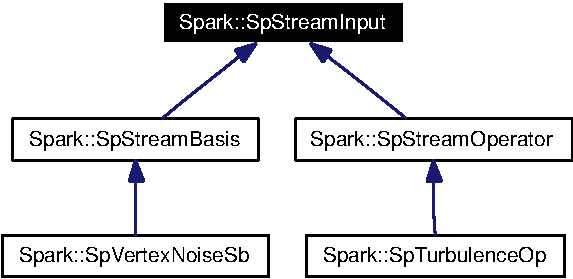
\includegraphics[width=155pt]{classSpark_1_1SpStreamInput__inherit__graph}
\end{center}
\end{figure}


\subsection{Detailed Description}
Abstract base class for an input stream for loading/generating a data stream. 

Definition at line 33 of file Sp\-Stream\-Input.h.\subsection*{Public Member Functions}
\begin{CompactItemize}
\item 
{\bf Sp\-Stream\-Input} ()
\begin{CompactList}\small\item\em Construction:. \item\end{CompactList}\item 
virtual {\bf $\sim$Sp\-Stream\-Input} ()
\item 
virtual bool {\bf has\-Changed} ()=0
\begin{CompactList}\small\item\em Methods:. \item\end{CompactList}\item 
virtual bool {\bf send\-Output\-To\-Buffer} ({\bf Sp\-Stream\-Buffer} $\ast$pk\-Buffer, {\bf Sp\-Stream\-Feedback} $\ast$pk\-Copy)=0
\end{CompactItemize}


\subsection{Constructor \& Destructor Documentation}
\index{Spark::SpStreamInput@{Spark::Sp\-Stream\-Input}!SpStreamInput@{SpStreamInput}}
\index{SpStreamInput@{SpStreamInput}!Spark::SpStreamInput@{Spark::Sp\-Stream\-Input}}
\subsubsection{\setlength{\rightskip}{0pt plus 5cm}Spark::Sp\-Stream\-Input::Sp\-Stream\-Input ()\hspace{0.3cm}{\tt  [inline]}}\label{classSpark_1_1SpStreamInput_a0}


Construction:. 

Definition at line 39 of file Sp\-Stream\-Input.h.\index{Spark::SpStreamInput@{Spark::Sp\-Stream\-Input}!~SpStreamInput@{$\sim$SpStreamInput}}
\index{~SpStreamInput@{$\sim$SpStreamInput}!Spark::SpStreamInput@{Spark::Sp\-Stream\-Input}}
\subsubsection{\setlength{\rightskip}{0pt plus 5cm}virtual Spark::Sp\-Stream\-Input::$\sim${\bf Sp\-Stream\-Input} ()\hspace{0.3cm}{\tt  [inline]}}\label{classSpark_1_1SpStreamInput_a1}


Definition at line 44 of file Sp\-Stream\-Input.h.

\subsection{Member Function Documentation}
\index{Spark::SpStreamInput@{Spark::Sp\-Stream\-Input}!hasChanged@{hasChanged}}
\index{hasChanged@{hasChanged}!Spark::SpStreamInput@{Spark::Sp\-Stream\-Input}}
\subsubsection{\setlength{\rightskip}{0pt plus 5cm}virtual bool Spark::Sp\-Stream\-Input::has\-Changed ()\hspace{0.3cm}{\tt  [pure virtual]}}\label{classSpark_1_1SpStreamInput_a2}


Methods:. 



Implemented in {\bf Spark::Sp\-Stream\-Basis} {\rm (p.\,\pageref{classSpark_1_1SpStreamBasis_a2})}, {\bf Spark::Sp\-Stream\-Operator} {\rm (p.\,\pageref{classSpark_1_1SpStreamOperator_a3})}, and {\bf Spark::Sp\-Vertex\-Noise\-Sb} {\rm (p.\,\pageref{classSpark_1_1SpVertexNoiseSb_a15})}.



Referenced by Spark::Sp\-Stream\-Operator::has\-Changed().\index{Spark::SpStreamInput@{Spark::Sp\-Stream\-Input}!sendOutputToBuffer@{sendOutputToBuffer}}
\index{sendOutputToBuffer@{sendOutputToBuffer}!Spark::SpStreamInput@{Spark::Sp\-Stream\-Input}}
\subsubsection{\setlength{\rightskip}{0pt plus 5cm}virtual bool Spark::Sp\-Stream\-Input::send\-Output\-To\-Buffer ({\bf Sp\-Stream\-Buffer} $\ast$ {\em pk\-Buffer}, {\bf Sp\-Stream\-Feedback} $\ast$ {\em pk\-Copy})\hspace{0.3cm}{\tt  [pure virtual]}}\label{classSpark_1_1SpStreamInput_a3}




Implemented in {\bf Spark::Sp\-Stream\-Basis} {\rm (p.\,\pageref{classSpark_1_1SpStreamBasis_a3})}, and {\bf Spark::Sp\-Stream\-Operator} {\rm (p.\,\pageref{classSpark_1_1SpStreamOperator_a4})}.



Referenced by Spark::Sp\-Turbulence\-Op::process\-Stream().

The documentation for this class was generated from the following file:\begin{CompactItemize}
\item 
{\bf Sp\-Stream\-Input.h}\end{CompactItemize}
